\section{Produktübersicht}
\setboolean{@twoside}{false}
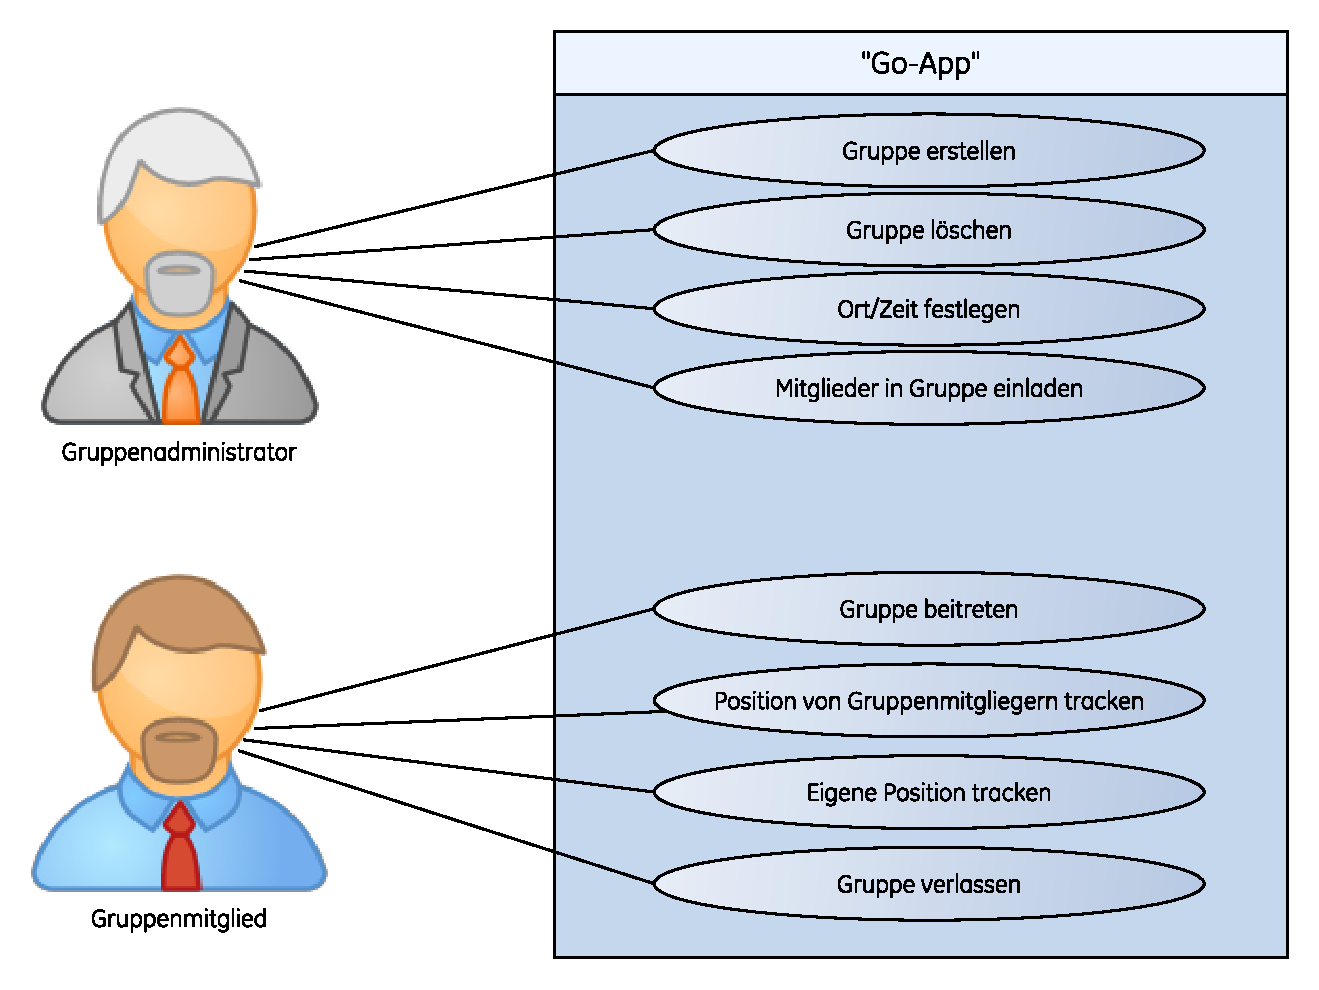
\includegraphics[scale=0.8, trim=2cm 0 0 0cm]{res/anwendungsfall.pdf}

\subsection{Systemarchitektur}

\begin{figure} [h]
	\centering
	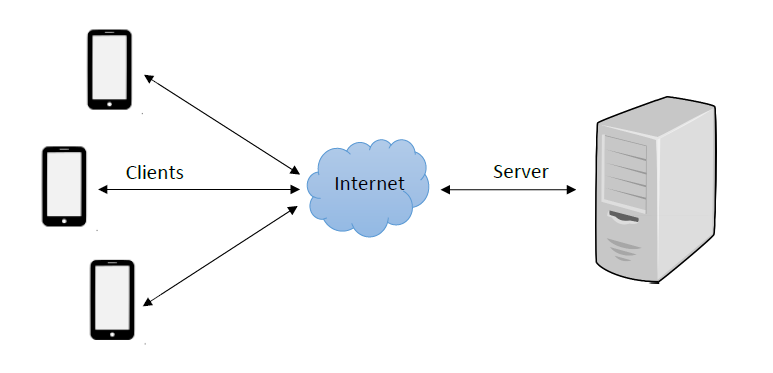
\includegraphics[scale = 0.8]{res/clientServerArchitektur.png}
\end{figure}
Die Client-Server-Architektur wird verwendet, da mehrere Mobiltelefone nebeneinander ohne konkrete Kenntnis voneinander zu haben, Ressourcen des Servers anfragen. Dieser wertet die Anfrage aus und liefert eine Antwort zurück an den Client. \\
In unserem Fall steht jeder Benutzer über einen zentralen Server in Verbindung mit seinen Gruppen und kann so z.B. die Standorte der anderen Mitglieder anfragen und bekommt diese dann vom Server geliefert.

\subsection{Szenarien}
\subsection{Szenario Kneipentour}
     Eine Person erstellt eine neue Gruppe und ist damit Administrator, kurz: Admin.\\
     Admin lädt Leute in die Gruppe ein via Share-Button. \\
     Danach sucht er den Zielort über die Suchzeile. Als er ihn gefunden hat, platziert er die Nadel darüber.\\
     Als nächstes setzt er den Zeitpunkt auf 21:00.\\
     Person2 bekommt die Einladung in Form von Link über einen Messenger zugesendet.\\
     Er tippt auf den Link und tritt der Gruppe bei. Er sieht den Zielpunkt und die Uhrzeit,\\
     kann diese aber nicht ändern.\\
     Um 20:55 drückt der Admin den Go-Button und macht sich auf den Weg zum Zielort.\\
     Person2 sieht den Admin auf der Karte und dass er losgelaufen ist. Person2 drückt ebenfalls auf "GO" und läuft ebenfalls los.\\
     Admin sieht, dass Person2 nur noch 100 Meter entfernt ist und wartet daher an einer geeigneten Stelle.\\
     Admin und Person2 treffen sich schon vor dem Ziel und gehen gemeinsam weiter.\\
     22:00: Der Admin setzt einen neuen Zielort "ClubX" und drückt den Go-Button.\\
     Person2 ist in ein wichtiges Telefonat verwickelt. Deshalb bekommt er nicht mit,\\
     dass der Admin schon weitergezogen ist.\\
     Person2 ist fertig und sucht nach dem Admin. Er öffnet die App und sieht, \\
     dass in der Gruppe ein neuer Zielort "ClubX" gesetzt wurde. Er sieht außerdem, dass der Admin bereits unterwegs ist.\\
     Person2 drückt erneut den Go-Button um dem Admin zu signalisieren, dass er zurückgeblieben ist.\\
     Danach macht er sich auf den Weg zum "ClubX" !!\\

\subsection{Anwendungsfälle}
\subsubsection{Musskriterien}
\subsubsection{Wunschkriterien}
